% Architecture of the risk-aware scheduler prototype on the OCUDU gNB.
% Column-width figure for acmart sigconf (\columnwidth = 241.1pt).
% Green marks the blocks of this work, white the stock OCUDU blocks, dashed blue the third-party ones.
% Build: pdflatex fig_ocudu_architecture.tex
\documentclass[tikz,border=1pt]{standalone}
\usepackage[T1]{fontenc}
\usepackage{libertine}
\usepackage[libertine]{newtxmath}
\usetikzlibrary{arrows.meta,positioning,calc}

\definecolor{ourfill}{HTML}{DDEFD9}   % this work (green family of the paper's plots)
\definecolor{ourline}{HTML}{2E7D32}
\definecolor{gnbfill}{HTML}{F1F3F5}
\definecolor{boxfill}{HTML}{FFFFFF}
\definecolor{extfill}{HTML}{E8EEF6}
\definecolor{extline}{HTML}{4A6FA5}
\definecolor{ink}{HTML}{222222}
\definecolor{soft}{HTML}{5F6B76}

\begin{document}
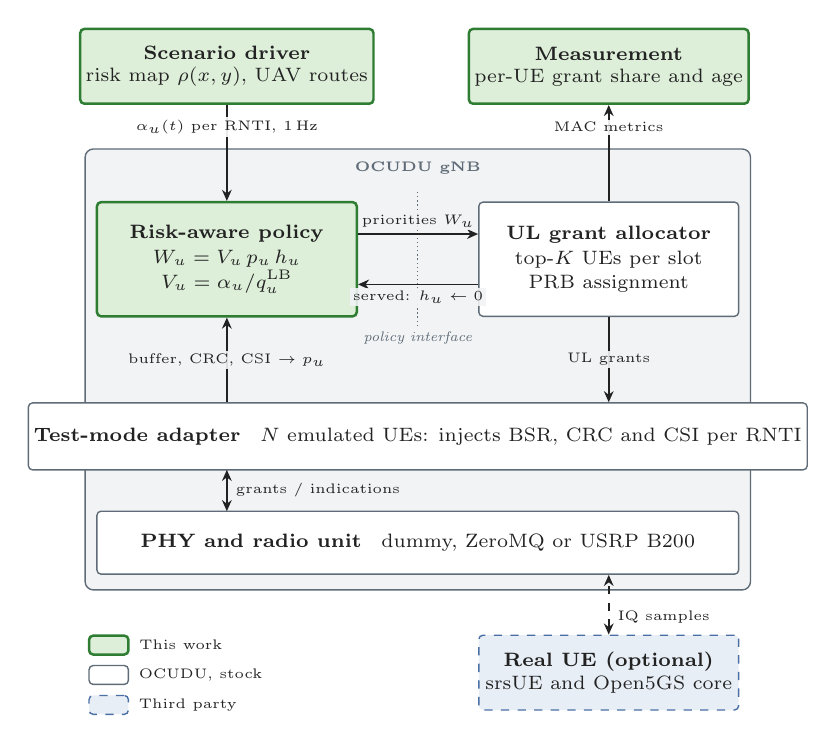
\begin{tikzpicture}[
    x=1cm, y=1cm, font=\scriptsize, text=ink,
    box/.style={line width=0.5pt, rounded corners=1.5pt, align=center, inner sep=2pt},
    stock/.style={box, draw=soft, fill=boxfill},
    ours/.style={box, draw=ourline, fill=ourfill, line width=0.9pt},
    third/.style={box, draw=extline, fill=extfill, dashed},
    flow/.style={-{Stealth[length=4pt,width=3.5pt]}, line width=0.6pt, draw=ink},
    lbl/.style={font=\tiny, text=ink, inner sep=1pt, fill=white, fill opacity=0.9, text opacity=1},
    lblg/.style={lbl, fill=gnbfill},
  ]

  % ---- OCUDU container ------------------------------------------------------
  \draw[draw=soft, line width=0.5pt, rounded corners=3pt, fill=gnbfill]
        (0,2.00) rectangle (8.45,7.60);
  \node[anchor=north, font=\tiny\bfseries, text=soft] at (4.225,7.56) {OCUDU gNB};

  % ---- this work, outside the gNB -------------------------------------------
  \node[ours, minimum width=3.3cm, minimum height=0.95cm] (drv) at (1.80,8.65)
       {\textbf{Scenario driver}\\ risk map $\rho(x,y)$, UAV routes};
  \node[ours, minimum width=3.3cm, minimum height=0.95cm] (met) at (6.65,8.65)
       {\textbf{Measurement}\\ per-UE grant share and age};

  % ---- inside the gNB -------------------------------------------------------
  \node[ours, minimum width=3.3cm, minimum height=1.45cm] (policy) at (1.80,6.20)
       {\textbf{Risk-aware policy}\\[1pt]
        $W_u = V_u\,p_u\,h_u$\\[1pt]
        $V_u = \alpha_u / q^{\mathrm{LB}}_u$};
  \node[stock, minimum width=3.3cm, minimum height=1.45cm] (alloc) at (6.65,6.20)
       {\textbf{UL grant allocator}\\[1pt]
        top-$K$ UEs per slot\\[1pt]
        PRB assignment};
  \node[stock, minimum width=8.15cm, minimum height=0.85cm] (tm) at (4.225,3.95)
       {\textbf{Test-mode adapter}\;\; $N$ emulated UEs: injects BSR, CRC and CSI per RNTI};
  \node[stock, minimum width=8.15cm, minimum height=0.80cm] (phy) at (4.225,2.60)
       {\textbf{PHY and radio unit}\;\; dummy, ZeroMQ or USRP B200};

  % ---- policy plug-in boundary ----------------------------------------------
  \draw[draw=soft, line width=0.5pt, densely dotted] (4.225,5.35) -- (4.225,7.05);
  \node[font=\tiny\itshape, text=soft, inner sep=1pt] at (4.225,5.20) {policy interface};

  % ---- third party ----------------------------------------------------------
  \node[third, minimum width=3.3cm, minimum height=0.95cm] (ue) at (6.65,0.95)
       {\textbf{Real UE (optional)}\\ srsUE and Open5GS core};

  % ---- flows ----------------------------------------------------------------
  \draw[flow] (drv.south) -- node[lbl, pos=0.23] {$\alpha_u(t)$ per RNTI, 1\,Hz} (policy.north);
  \draw[flow] (alloc.north) -- node[lbl, pos=0.77] {MAC metrics} (met.south);

  \draw[flow] ([yshift=0.32cm]policy.east) -- node[lblg, above=1pt] {priorities $W_u$}
              ([yshift=0.32cm]alloc.west);
  \draw[flow] ([yshift=-0.32cm]alloc.west) -- node[lblg, below=1pt] {served: $h_u \leftarrow 0$}
              ([yshift=-0.32cm]policy.east);

  \draw[flow] (alloc.south) -- node[lblg, pos=0.5] {UL grants} (alloc.south |- tm.north);
  \draw[flow] (policy.south |- tm.north) -- node[lblg, pos=0.5] {buffer, CRC, CSI $\rightarrow p_u$}
              (policy.south);

  \draw[flow, {Stealth[length=4pt,width=3.5pt]}-{Stealth[length=4pt,width=3.5pt]}] (1.80,3.00) -- node[lblg, right=2pt] {grants / indications} (1.80,3.525);
  \draw[flow, dashed, {Stealth[length=4pt,width=3.5pt]}-{Stealth[length=4pt,width=3.5pt]}] (ue.north) -- node[lbl, right=2pt, pos=0.3] {IQ samples} (ue.north |- phy.south);

  % ---- legend ---------------------------------------------------------------
  \begin{scope}[font=\tiny]
    \node[ours,  minimum width=0.5cm, minimum height=0.24cm, inner sep=0pt] (l1) at (0.30,1.30) {};
    \node[anchor=west] at (l1.east) {This work};
    \node[stock, minimum width=0.5cm, minimum height=0.24cm, inner sep=0pt] (l2) at (0.30,0.92) {};
    \node[anchor=west] at (l2.east) {OCUDU, stock};
    \node[third, minimum width=0.5cm, minimum height=0.24cm, inner sep=0pt] (l3) at (0.30,0.54) {};
    \node[anchor=west] at (l3.east) {Third party};
  \end{scope}
\end{tikzpicture}
\end{document}
